% Options for packages loaded elsewhere
% Options for packages loaded elsewhere
\PassOptionsToPackage{unicode}{hyperref}
\PassOptionsToPackage{hyphens}{url}
\PassOptionsToPackage{dvipsnames,svgnames,x11names}{xcolor}
%
\documentclass[
]{standalone}
\usepackage{xcolor}
\usepackage{amsmath,amssymb}
\setcounter{secnumdepth}{-\maxdimen} % remove section numbering
\usepackage{iftex}
\ifPDFTeX
  \usepackage[T1]{fontenc}
  \usepackage[utf8]{inputenc}
  \usepackage{textcomp} % provide euro and other symbols
\else % if luatex or xetex
  \usepackage{unicode-math} % this also loads fontspec
  \defaultfontfeatures{Scale=MatchLowercase}
  \defaultfontfeatures[\rmfamily]{Ligatures=TeX,Scale=1}
\fi
\usepackage{lmodern}
\ifPDFTeX\else
  % xetex/luatex font selection
\fi
% Use upquote if available, for straight quotes in verbatim environments
\IfFileExists{upquote.sty}{\usepackage{upquote}}{}
\IfFileExists{microtype.sty}{% use microtype if available
  \usepackage[]{microtype}
  \UseMicrotypeSet[protrusion]{basicmath} % disable protrusion for tt fonts
}{}
\makeatletter
\@ifundefined{KOMAClassName}{% if non-KOMA class
  \IfFileExists{parskip.sty}{%
    \usepackage{parskip}
  }{% else
    \setlength{\parindent}{0pt}
    \setlength{\parskip}{6pt plus 2pt minus 1pt}}
}{% if KOMA class
  \KOMAoptions{parskip=half}}
\makeatother
% Make \paragraph and \subparagraph free-standing
\makeatletter
\ifx\paragraph\undefined\else
  \let\oldparagraph\paragraph
  \renewcommand{\paragraph}{
    \@ifstar
      \xxxParagraphStar
      \xxxParagraphNoStar
  }
  \newcommand{\xxxParagraphStar}[1]{\oldparagraph*{#1}\mbox{}}
  \newcommand{\xxxParagraphNoStar}[1]{\oldparagraph{#1}\mbox{}}
\fi
\ifx\subparagraph\undefined\else
  \let\oldsubparagraph\subparagraph
  \renewcommand{\subparagraph}{
    \@ifstar
      \xxxSubParagraphStar
      \xxxSubParagraphNoStar
  }
  \newcommand{\xxxSubParagraphStar}[1]{\oldsubparagraph*{#1}\mbox{}}
  \newcommand{\xxxSubParagraphNoStar}[1]{\oldsubparagraph{#1}\mbox{}}
\fi
\makeatother


\usepackage{longtable,booktabs,array}
\usepackage{calc} % for calculating minipage widths
% Correct order of tables after \paragraph or \subparagraph
\usepackage{etoolbox}
\makeatletter
\patchcmd\longtable{\par}{\if@noskipsec\mbox{}\fi\par}{}{}
\makeatother
% Allow footnotes in longtable head/foot
\IfFileExists{footnotehyper.sty}{\usepackage{footnotehyper}}{\usepackage{footnote}}
\makesavenoteenv{longtable}
\usepackage{graphicx}
\makeatletter
\newsavebox\pandoc@box
\newcommand*\pandocbounded[1]{% scales image to fit in text height/width
  \sbox\pandoc@box{#1}%
  \Gscale@div\@tempa{\textheight}{\dimexpr\ht\pandoc@box+\dp\pandoc@box\relax}%
  \Gscale@div\@tempb{\linewidth}{\wd\pandoc@box}%
  \ifdim\@tempb\p@<\@tempa\p@\let\@tempa\@tempb\fi% select the smaller of both
  \ifdim\@tempa\p@<\p@\scalebox{\@tempa}{\usebox\pandoc@box}%
  \else\usebox{\pandoc@box}%
  \fi%
}
% Set default figure placement to htbp
\def\fps@figure{htbp}
\makeatother





\setlength{\emergencystretch}{3em} % prevent overfull lines

\providecommand{\tightlist}{%
  \setlength{\itemsep}{0pt}\setlength{\parskip}{0pt}}



 


% preamble.tex
\usepackage{tikz}
\usepackage{xcolor}
\usetikzlibrary{positioning,arrows.meta,fit}
\tikzset{>=Stealth}

% Farger
\definecolor{cTop}{RGB}{230,170,160}
\definecolor{cInvest}{RGB}{32,75,111}
\definecolor{cFinance}{RGB}{146,185,221}
\definecolor{cPayout}{RGB}{0,128,128}
\makeatletter
\@ifpackageloaded{caption}{}{\usepackage{caption}}
\AtBeginDocument{%
\ifdefined\contentsname
  \renewcommand*\contentsname{Table of contents}
\else
  \newcommand\contentsname{Table of contents}
\fi
\ifdefined\listfigurename
  \renewcommand*\listfigurename{List of Figures}
\else
  \newcommand\listfigurename{List of Figures}
\fi
\ifdefined\listtablename
  \renewcommand*\listtablename{List of Tables}
\else
  \newcommand\listtablename{List of Tables}
\fi
\ifdefined\figurename
  \renewcommand*\figurename{Figure}
\else
  \newcommand\figurename{Figure}
\fi
\ifdefined\tablename
  \renewcommand*\tablename{Table}
\else
  \newcommand\tablename{Table}
\fi
}
\@ifpackageloaded{float}{}{\usepackage{float}}
\floatstyle{ruled}
\@ifundefined{c@chapter}{\newfloat{codelisting}{h}{lop}}{\newfloat{codelisting}{h}{lop}[chapter]}
\floatname{codelisting}{Listing}
\newcommand*\listoflistings{\listof{codelisting}{List of Listings}}
\makeatother
\makeatletter
\makeatother
\makeatletter
\@ifpackageloaded{caption}{}{\usepackage{caption}}
\@ifpackageloaded{subcaption}{}{\usepackage{subcaption}}
\makeatother
\usepackage{bookmark}
\IfFileExists{xurl.sty}{\usepackage{xurl}}{} % add URL line breaks if available
\urlstyle{same}
\hypersetup{
  colorlinks=true,
  linkcolor={blue},
  filecolor={Maroon},
  citecolor={Blue},
  urlcolor={Blue},
  pdfcreator={LaTeX via pandoc}}


\author{}
\date{}
\begin{document}


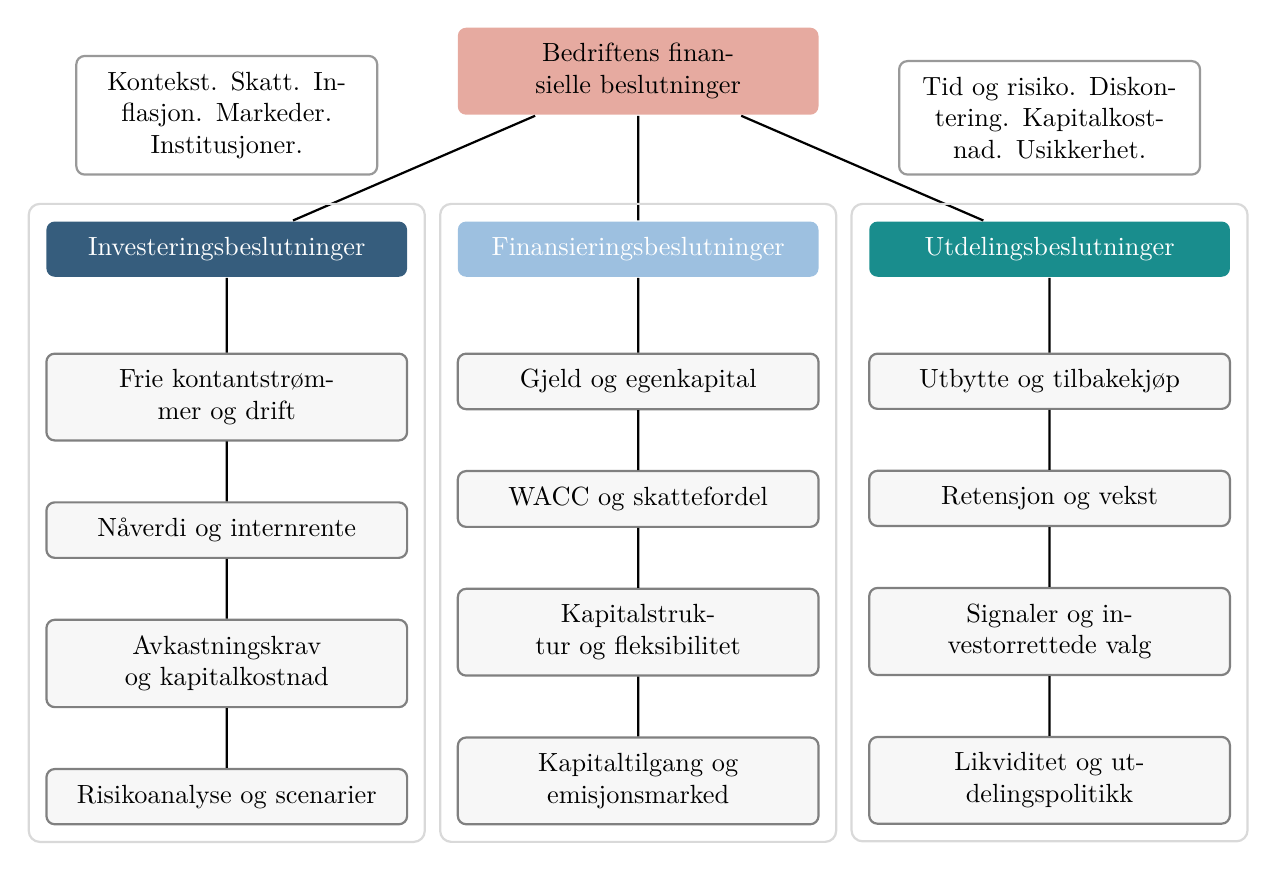
\begin{tikzpicture}[
  scale=0.95,
  every node/.style={transform shape},
  thick,
  node distance=8mm and 12mm
]

% Farger.
\definecolor{cTop}{RGB}{230,170,160}
\definecolor{cInvest}{RGB}{32,75,111}
\definecolor{cFinance}{RGB}{146,185,221}
\definecolor{cPayout}{RGB}{0,128,128}
\definecolor{cContext}{RGB}{240,200,160}
\definecolor{cRisk}{RGB}{200,160,200}

% Stiler.
\tikzset{
  box/.style={rectangle, rounded corners=3pt, inner sep=6pt, align=center, text width=44mm},
  lvlA/.style={box, fill=cTop, text=black},
  lvlB/.style={box, fill=black!3, draw=black!50, text=black},
  colInvest/.style={fill=cInvest!90, text=white},
  colFinance/.style={fill=cFinance!90, text=white},
  colPayout/.style={fill=cPayout!90, text=white},
  side/.style={box, draw=black!40, fill=white, text=black, text width=36mm}
}

% Topp.
\node (top) [lvlA] {Bedriftens finansielle beslutninger};

% Nivå 2.
\node (invest)  [box,colInvest, below=14mm of top, xshift=-55mm] {Investeringsbeslutninger};
\node (finance) [box,colFinance, below=14mm of top]               {Finansieringsbeslutninger};
\node (payout)  [box,colPayout,  below=14mm of top, xshift=55mm]  {Utdelingsbeslutninger};

% Piler topp til nivå 2.
\draw[thick] (top) -- (invest);
\draw[thick] (top) -- (finance);
\draw[thick] (top) -- (payout);

% Nivå 3 under Investering.
\node (inv1) [lvlB, below=of invest, yshift=-2mm] {Frie kontantstrømmer og drift};
\node (inv2) [lvlB, below=of inv1] {Nåverdi og internrente};
\node (inv3) [lvlB, below=of inv2] {Avkastningskrav og kapitalkostnad};
\node (inv4) [lvlB, below=of inv3] {Risikoanalyse og scenarier};

% Nivå 3 under Finansiering.
\node (fin1) [lvlB, below=of finance, yshift=-2mm] {Gjeld og egenkapital};
\node (fin2) [lvlB, below=of fin1] {WACC og skattefordel};
\node (fin3) [lvlB, below=of fin2] {Kapitalstruktur og fleksibilitet};
\node (fin4) [lvlB, below=of fin3] {Kapitaltilgang og emisjonsmarked};

% Nivå 3 under Utdeling.
\node (pay1) [lvlB, below=of payout, yshift=-2mm] {Utbytte og tilbakekjøp};
\node (pay2) [lvlB, below=of pay1] {Retensjon og vekst};
\node (pay3) [lvlB, below=of pay2] {Signaler og investorrettede valg};
\node (pay4) [lvlB, below=of pay3] {Likviditet og utdelingspolitikk};

% Piler nivå 2 til nivå 3.
\foreach \a/\b in {invest/inv1, inv1/inv2, inv2/inv3, inv3/inv4,
                   finance/fin1, fin1/fin2, fin2/fin3, fin3/fin4,
                   payout/pay1, pay1/pay2, pay2/pay3, pay3/pay4}{
  \draw[thick] (\a) -- (\b);
}

% Sidebokser for kontekst og for tid og risiko.
\node (context) [side, left=50mm of finance, above=of invest, yshift=-2mm] {Kontekst. Skatt. Inflasjon. Markeder. Institusjoner.};
\node (risk)    [side, right=50mm of finance, above=of payout, yshift=-2mm] {Tid og risiko. Diskontering. Kapitalkostnad. Usikkerhet.};

% Diskret rammer som grupperer hver søyle.
\node[draw=black!15, rounded corners=4pt, fit=(invest) (inv4), inner sep=6pt] {};
\node[draw=black!15, rounded corners=4pt, fit=(finance) (fin4), inner sep=6pt] {};
\node[draw=black!15, rounded corners=4pt, fit=(payout) (pay4), inner sep=6pt] {};
\end{tikzpicture}




\end{document}
